\subsection{Red corporativa de empresa de Telecomunicaciones - Captura wireless}

Esta red nos presentó desafíos particularmente interesantes, se trata de una red wireless corporativa de una empresa de telecomunicaciones con una infraestructura que puede ser típica pero nos resultó anti-intuitiva. La red y el entorno de captura eran particularmente activos y se efectuó la captura durante 35 minutos aproximadamente.

El enfoque ingenuo que utilizamos a priori nos generó cantidades de información imposibles de analizar y gráficos francamente incomprensibles, esto nos llevo a los refinamientos de agrupación de nodos (sumarización de redes) y distinción visual por colores y tamaños explicados en la sección desarrollo.

A continuación se aprecia el gráfico generado para s1 modelada como la fuente que distingue paquetes \textit{Who-has} de acuerdo a la ip de origen del paquete

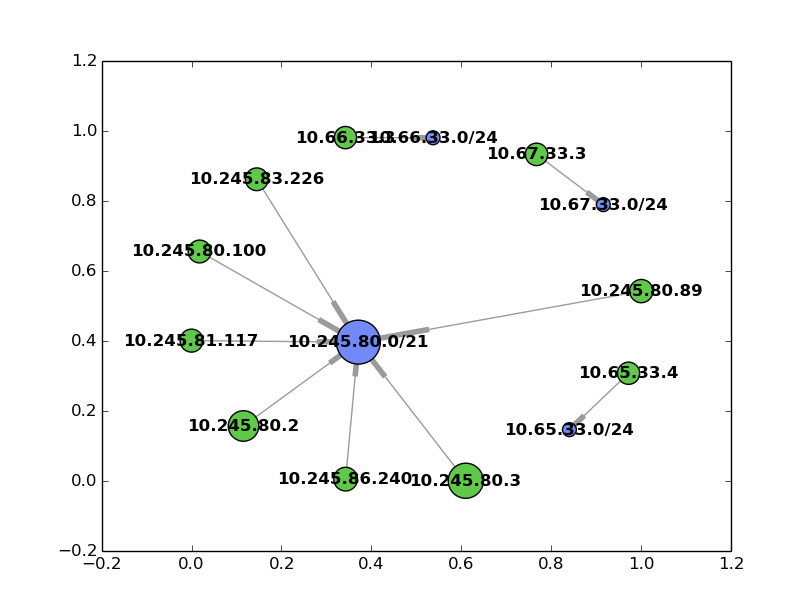
\includegraphics[scale=0.80]{imagenes/TCORP-wireless.png}

Puede verse en la componente conexa más grande del grafo que los nodos distinguidos más grandes son el 10.245.80.2 y 10.245.80.3, hipotetizamos de acuerdo a nuestro modelo que esos dos nodos juegan el papel de default gateway en la red. Sabemos también a priori que la ip del equipo que efectuó la captura es 10.245.80.89.

Nos llamó la atención que el equipo que efectua la captura no tenga interacción con los gateways, asi como tampoco el resto de los nodos distinguidos que aportan una cantidad de información similar a la capturadora. 

A lo largo de todo el desarrollo partimos del supuesto que los paquetes \textit{Who-has} eran la clave del modelado debido al principio teórico que manifiesta que todos los nodos actualizan sus tablas ARP utilizando paquetes de este tipo y siguiendo la idea que aquellos nodos que más actividad expresaban eran los default gateways dado que debían mantener información sobre toda la LAN, pero además sabemos que cada nodo debe actualizar la información sobre su default gateway de la misma manera, con lo que la ausencia de conexiones entre los equipos calificados como distinguidos con sus default gateways nos pareció una inconsistencia importante.

Indagando un poco más en la configuración de la capturadora, nos encontramos que por si esta inconsistencia no fuera suficiente, el default gateway que tenía configurada era un nodo que ni siquiera califica como distinguido, aquel cuya ip es 10.245.80.1 (que queda agrupado dentro de la nube de nodos no distinguidos). 

Llegados a este punto del análisis acudimos a metodologías experimentales y no tanto para arrojar más luz sobre la topología de la red, que pasamos a detallar.

Primero analizamos los datos arrojados por una fuente de información alternativa, particularmente, la fuente que distingue mensajes \textit{Who-has} basados en la ip destino. A pesar de las estrategias de agrupación de nodos y dimensionamiento en base a cantidad de información el gráfico generado es muy complejo para analizar a simple vista y decidimos no incluirlo, baste declarar que efectivamente aparece como nodo distinguido el default gateway declarado (10.245.80.1) pero su tamaño es sólo marginalmente mayor que el del resto de los nodos distinguidos hallados, y siendo estos notablemente más que para la fuente original, se dificulta hallarlo en una inspeción visual.

% Posterior al análisis experimental
Para complementar el análisis puramente experimental acudimos a enfoques alternativos tales como analizar los nodos distinguidos con otras herramientas, especificamente \textit{nmap} para verificar hipótesis sobre cuales eran los verdaderos gateways y cuales eran equipos normales que sólo calificaban como nodos distinguidos debido a su actividad excesiva en relación con los nodos no distinguidos. Basados en la detección de sistema operativo que ofrece, confirmamos que los nodos distinguidos 10.245.80.2 y 10.245.80.3 eran efectivamente elementos de red, dado que sus sistemas operativos eran \textit{Cisco iOS}, adicionalmente se confirmó que el resto de los nodos distinguidos dentro de la componente conexa que estamos analizando eran equipos de usuario final, en general con alguna variante de sistema operativo Windows y reforzados por los hostnames descubiertos que seguian la nomenclatura estricta de los equipos pertenecientes al dominio corporativo en la empresa. El análisis mediante nmap del default gateway declarado arrojó que el nodo no respondía con ninguna información útil.

La hipótesis a la que arribamos, luego de comentar la situación con expertos en el lugar de la captura, fue que probablemente la ip 10.245.80.1 perteneciera a un balanceador de carga /una especie de ip virtual) que distribuyera la misma entre dos nodos físicos: 10.245.80.2 y 10.245.80.3, esto explica tambien la ausencia de conexiones entre los nodos distinguidos que resultaron ser PCs de usuarios finales y los gateways descubiertos, dado que los paquetes \textit{Who-has} de estos nodos para actualizar la MAC de su default gateway fueron efectuados hacia la 10.245.80.1 (que queda oculta dentro de la nube) mientras que la actualización de las tablas ARP de los default gateways físicos, se generaba con origen ip de las ips físicas de dichos nodos.

Esto aún dejaba la duda de por qué los gateways físicos no actualizaban la información del resto de los nodos distinguidos, nuestra conclusión es que al experimentar mucho tráfico (el tráfico suficiente para que califique como nodo distinguido) y debido a la naturaleza asimetrica de la red en cuestión, la capturadora generó mucho trafico preguntando por su default gateway declarado 10.245.80.1 (que es una ip de balanceo descargando sobre 10.245.80.2 y 10.245.80.3  que como puede apreciarse por los tamaños de esos nodos en el grafico son aquellos nodos más distinguidos - aquellos con mayor actividad): la tabla ARP de los gateways resetea su tiempo de vida en relación al nodo que efectua la captura, haciendo innecesario que los gateways salgan a preguntar a toda la red, quien posee la dirección ip 10.245.80.89.
Similarmente arribamos a una conclusión paralela para el resto de los nodos distinguidos que registra menor actividad que los gateways.

También se confirmó esta hipótesis averiguando con los encargados del diseño, implementación y mantenimiento de la red, quienes verificaron que los gateways principales en la red eran los nodos 10.245.80.2 y 10.245.80.3 para la red de mayor actividad, que es a la que el equipo capturador se encontraba asociada (y adicionalmente aquella cuyo rango de potencia de radio era más fuerte debido a la cantidad de actividad mayor que se registró). También nos indicaron que por política de la empresa las primeras 15 ips disponibles de cada red se reservaban para la utilización a discreción del grupo de networking.

Pueden observarse superpuestas en el grafico redes de menor tamaño y trafico en los que la evidencia experimental (y la investigación de la infraestructura llevada a cabo) para lo que ocurre lo mismo: los gateways están dentro de los primeros 15 hosts de la red (reservados por el grupo de networking en todas las redes corporativas), en particular en los x.x.x.3 y x.x.x.4 y actualizan su tabla respecto de hosts que estan en sus redes (10.65.33.0/24, 10.66.33.0/24 y 10.67.33.0/24)